\documentclass[crop, tikz]{standalone}

\usepackage{tikz}

\usepackage[sfdefault, light]{FiraSans}

\begin{document}


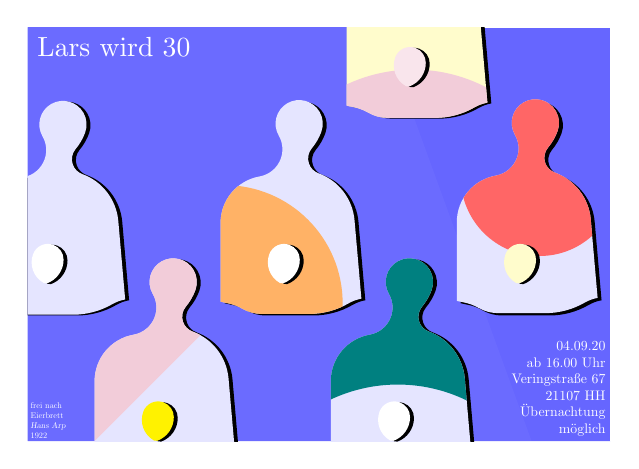
\begin{tikzpicture}


\def\sil{
--++(0,1)arc(180:100:.6)arc(-80:30:.35)arc(210:-20:.3)arc(-20:-40:.7)arc(140:250:.2)arc(70:5:.7)--++(275:1)arc(100:120:.5)arc(300:270:1)--++(-.6,0)arc(270:240:.5)arc(60:80:.6)--cycle;
}
\def\egg{
arc(240:160:.3)arc(160:0:.2)arc(0:-70:.32)arc(-70:-120:.05)--cycle
}


% Die DIN A6-Maße sind 14,8 cm mal 10,5 cm
\clip (1/2,7/2)coordinate(1)rectangle(15.8/2, -3.5/2)coordinate(2);
\fill[fill=blue!60] (1)rectangle(2);

\fill[fill=blue!58] (2)++(-1,0)--++(-4,11)--(1)|-(2);



%%% 1
\fill[black] (0,0) \sil ;
\fill[blue!10] (-.05,.01) \sil ;
\fill[black] (.75,.25) \egg;
\fill[white] (.7,.26) \egg;



%%% 2
\begin{scope}[xshift=3cm]
\fill[black] (0,0) \sil ;
\fill[blue!10] (-.05,.02) \sil ;
\begin{scope}[]
	\clip (0,0)circle(1.5);
	\fill[orange!60] (-.05,.02) \sil ;
\end{scope}
\fill[black] (.75,.25) \egg;
\fill[white] (.7,.26) \egg;
\end{scope}

%%% 3
\begin{scope}[xshift=6cm]
\fill[black] (0,0) \sil ;
\fill[blue!10] (-.05,.03) \sil ;
\begin{scope}[]
	\clip (1,1.6)circle(1.);
	\fill[red!60] (-.05,.03) \sil ;
\end{scope}
\fill[black] (.75,.25) \egg;
\fill[yellow!20] (.7,.26) \egg;
\end{scope}


%%% 4
\begin{scope}[xshift=1.4cm, yshift=-2cm]
\fill[black] (0,0) \sil ;
\fill[blue!10] (-.05,.01) \sil ;
\begin{scope}[]
	\clip (-.2,.1)--++(45:4)--++(180:5);
	\fill[purple!20] (-.05,.01) \sil ;
\end{scope}
\fill[black] (.75,.25) \egg;
\fill[yellow] (.7,.26) \egg;
\end{scope}



%%% 5
\begin{scope}[xshift=4.4cm, yshift=-2cm]
\fill[black] (0,0) \sil ;
\fill[blue!10] (-.05,.01) \sil ;
\begin{scope}[]
	\clip (-.2,.7)arc(120:60:2)--++(90:5)--++(180:5);
	\fill[green!50!blue] (-.05,.01) \sil ;
\end{scope}
\fill[black] (.75,.25) \egg;
\fill[white] (.7,.26) \egg;
\end{scope}

%%% 6
\begin{scope}[xshift=4.6cm, yshift=2.5cm]
\fill[black] (0,0) \sil ;
\fill[yellow!20] (-.05,.01) \sil ;
\begin{scope}[]
	\clip (-.2,.2)arc(120:60:2)--++(-90:5)--++(180:5);
	\fill[purple!20] (-.05,.01) \sil ;
\end{scope}
\fill[black] (.75,.25) \egg;
\fill[purple!10] (.7,.26) \egg;
\end{scope}



%% Text
%\path (1) node[below right, white]{
%Herzliche Einladung zur Geburtstagsparty
%};

%\path (1) node[below right, white, align=left]{
%Herzliche Einladung zum snacken und sippen \\ 
%anlässlich der 30
%};

\path (1) node[below right, white, align=left]{
Lars wird 30
};

\path (2) node[above left, white, align=right, scale=.5]{
04.09.20 \\ ab 16.00 Uhr \\ Veringstraße 67 \\ 21107 HH \\ Übernachtung \\ möglich
};

\path (1)|-(2) node[midway, above right, scale=.3, align=left, white]{frei nach \\ Eierbrett \\ \textsl{Hans Arp} \\ 1922};


\end{tikzpicture}
\end{document}